\chapter{FlexoGraph API Usage Examples}
\label{chap:appendix:api}

This appendix provides code examples illustrating how applications interact with the \project{} API introduced in~\autoref{arch:api}.
\autoref{appendix:anatomy} shows the basic structure of a \project{} application, and~\autoref{appendix:iterators} describes the iterator class hierarchy.
\autoref{appendix:pagerank_graphapi} shows how the PageRank algorithm from~\autoref{alg:PageRankPullGS} is implemented using the \api{}.

%%%%%%%%%%%%%%%%%%%%%%%%%%%%%%%%%%%%%%%%%%%%%%%%%%%%%%%%%%%%%%%%%%%%%%%%%%%%%%%%
\section{Anatomy of a \project{} Application}
\label{appendix:anatomy}

\autoref{lst:flexographApp} shows a minimal application that traverses the out-neighborhood of every vertex in parallel.
The three highlighted regions correspond to the three architectural layers: the \highlightP{engine} layer, the \highlightB{graph handle} layer, and the \highlightM{cursor} layer.

\begin{lstlisting}[style=cpp,label=lst:flexographApp,caption={Example application using the \api{} to scan out-neighborhoods in parallel.  \highlightP{GraphEngine} owns the connection and computes partitions; \highlightB{GraphBase} provides a per-thread handle; \highlightM{OutCursor} iterates a partition's neighborhoods.},captionpos=b]
(*@\highlightP{GraphEngine graphEngine(num\_threads, engine\_opts);}@*)
(*@\highlightP{graphEngine.calculate\_thread\_offsets();}@*)
#pragma omp parallel for
for (int i = 0; i < num_threads; i++)
{
  (*@\highlightB{GraphBase* graph = graphEngine.create\_graph\_handle();}@*)
  (*@\highlightB{adjlist found;}@*)

  (*@\highlightM{OutCursor* out\_cursor = graph->get\_outnbd\_iter();}@*)
  (*@\highlightM{out\_cursor->set\_key\_range(graphEngine.get\_key\_range(i));}@*)
  (*@\highlightM{out\_cursor->next(\&found);}@*)
  while (found.node_id != OutOfBand_ID_MAX)
  {
      for (node_id_t v : found.edgelist)
      {
          // process edge (found.node_id -> v)
      }
      out_cursor->next(&found);
  }
  out_cursor->close();
  graph->close();
}
\end{lstlisting}

An application begins by creating a \highlightP{\code{GraphEngine}} object (line~1), which opens the \wt{} connection and reads the graph metadata.
A call to \code{calculate\_thread\_offsets()} (line~2) partitions the vertex ID space into disjoint key ranges using the active partitioning strategy (\autoref{arch:api:partitioning}).

Inside the OpenMP parallel region, each thread creates its own \highlightB{\code{GraphBase}} handle (line~6) via \code{create\_graph\_handle()}.
This handle encapsulates a private \wt{} session and the cursors needed to access the graph tables; because sessions and cursors are not thread-safe in \wt{}, each thread must have its own handle.

The thread then obtains an \highlightM{\code{OutCursor}} (line~9), sets its key range to the thread's assigned partition (line~10), and begins iterating.
Each call to \code{next()} (lines~11, 17) populates the \code{adjlist} struct with the next vertex's ID, degree, and neighbor list.
When the cursor reaches the end of its partition, it sets \code{found.node\_id} to the out-of-band sentinel, terminating the loop.

%%%%%%%%%%%%%%%%%%%%%%%%%%%%%%%%%%%%%%%%%%%%%%%%%%%%%%%%%%%%%%%%%%%%%%%%%%%%%%%%
\section{Iterator Class Hierarchy}
\label{appendix:iterators}

\autoref{lst:table_iterator} shows the \code{table\_iterator} base class from which all topology cursors inherit.
The base class wraps a \wt{} cursor and session, tracks whether the cursor has been positioned (\code{is\_first}) and whether more elements remain (\code{has\_next}), and provides \code{reset()} and \code{close()} methods.

\begin{figure*}[h!]
\begin{minipage}{0.48\textwidth}
\begin{lstlisting}[style=cpp,label={lst:table_iterator},caption={\code{table\_iterator} base class.},captionpos=b]
class table_iterator
{
protected:
  WT_CURSOR *cursor = nullptr;
  WT_SESSION *session = nullptr;
  bool is_first = true;
  bool has_next = true;

public:
  table_iterator() = default;
  virtual ~table_iterator() = default;
  bool has_more() const
    { return has_next; };
  virtual void reset()
  {
    cursor->reset(cursor);
    is_first = true;
    has_next = true;
  }
  void close()
    { cursor->close(cursor); }
};
\end{lstlisting}
\end{minipage}
\hfill
\begin{minipage}{0.48\textwidth}
\centering
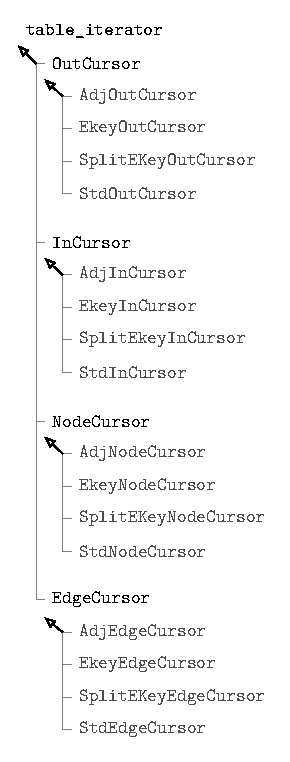
\includegraphics[width=\textwidth]{fig/appendix/iterator_inherit_graph.pdf}
\captionof{figure}{Inheritance hierarchy for the topology cursor classes.  Each representation provides concrete implementations (e.g., \code{AdjOutCursor}, \code{SplitEKeyOutCursor}) of the four abstract cursor types.}
\label{fig:iterator_diagram}
\end{minipage}
\end{figure*}

The four abstract cursor subclasses --- \code{OutCursor}, \code{InCursor}, \code{NodeCursor}, and \code{EdgeCursor} --- each add a \code{set\_key\_range()} method and a \code{next()} method whose signature matches the element type (\code{adjlist*} for neighborhood cursors, \code{node*} for node cursors, \code{edge*} for edge cursors).
Each representation provides a concrete implementation of these cursors:
\begin{itemize}
  \item \code{AdjOutCursor} positions the \wt{} cursor at the adjacency table entry for the current vertex and deserializes neighbor IDs from the packed blob, advancing to the next vertex when the blob is exhausted.
  \item \code{SplitEKeyOutCursor} simply advances the \wt{} cursor to the next key in the B-tree; each key is one edge, so \code{next()} is a single cursor step.
\end{itemize}
The application interacts only with the abstract cursor types returned by the factory methods in~\autoref{tab:graphapi}, so cursor usage is identical regardless of the underlying representation.

%%%%%%%%%%%%%%%%%%%%%%%%%%%%%%%%%%%%%%%%%%%%%%%%%%%%%%%%%%%%%%%%%%%%%%%%%%%%%%%%
\section{PageRank Implementation}
\label{appendix:pagerank_graphapi}

\autoref{lst:pagerank_graphapi} shows the GAPBS PageRank kernel~\cite{beamer2015gap} adapted to use the \api{}.
The structure mirrors the pseudocode in~\autoref{alg:PageRankPullGS}: a degree-initialization pass using \code{NodeCursor}, followed by iterative score updates using \code{InCursor}.

\begin{lstlisting}[style=cpp, label={lst:pagerank_graphapi}, caption={GAPBS PageRank kernel adapted to use the \api{}.  Each thread creates its own \code{GraphBase} handle and cursors, scoped to a disjoint partition.}, captionpos=b]
pvector<ScoreT> pagerank(GraphEngine& graph_engine,
                         int num_threads,
                         int max_iters,
                         node_id_t num_nodes,
                         node_id_t max_node_id,
                         double epsilon = 0)
{
    pvector<ScoreT> src(max_node_id, 0);
    pvector<ScoreT> dst(max_node_id, 1.0 / num_nodes);
    pvector<node_id_t> deg(max_node_id, 0);

    // Phase 1: collect out-degrees
    #pragma omp parallel for
    for (int i = 0; i < num_threads; i++)
    {
        GraphBase* graph = graph_engine.create_graph_handle();
        NodeCursor* node_cursor = graph->get_node_iter();
        node_cursor->set_key_range(graph_engine.get_key_range(i));

        node found = {0};
        node_cursor->next(&found);
        while (found.id != OutOfBand_ID_MAX)
        {
            deg[found.id] = found.out_degree;
            node_cursor->next(&found);
        }
        node_cursor->close();
        graph->close(false);
    }

    // Phase 2: iterative score updates
    for (int iter = 0; iter < max_iters; iter++)
    {
        double error = 0;
        #pragma omp parallel for reduction(+ : error)
        for (int i = 0; i < num_threads; i++)
        {
            GraphBase* graph = graph_engine.create_graph_handle();
            InCursor* in_cursor = graph->get_innbd_iter();
            in_cursor->set_key_range(graph_engine.get_key_range(i));

            adjlist found;
            in_cursor->next(&found);
            while (found.node_id != OutOfBand_ID_MAX)
            {
                ScoreT incoming_total = 0;
                for (node_id_t v : found.edgelist)
                {
                    incoming_total += src[v];
                }

                ScoreT old_score = dst[found.node_id];
                dst[found.node_id] =
                    (1 - kDamp) / num_nodes + kDamp * incoming_total;
                error += fabs(dst[found.node_id] - old_score);
                src[found.node_id] =
                    dst[found.node_id] / deg[found.node_id];

                in_cursor->next(&found);
            }
            in_cursor->close();
            graph->close(false);
        }
        if (error < epsilon) break;
    }
    return dst;
}
\end{lstlisting}

The key adaptations from the original GAPBS implementation are:
\begin{itemize}
  \item OpenMP's automatic loop parallelization cannot be used directly because each thread must construct its own \code{GraphBase} handle and cursors. Instead, the loop is parallelized manually, with each thread obtaining its partition via \code{get\_key\_range()}.
  \item The \code{pvector} utility class (from GAPBS) supports parallel initialization; \project{} extends it to use an \code{mmap}-backed buffer so that computed scores can be persisted across runs without a separate serialization step.
\end{itemize}
